\newpage
\section{Análisis y diseño del sistema}
\noindent En esta sección se especificarán los casos de uso que componen el sistema, además de los requisitos funcionales y no funcionales para ambas clasificaciones, estática y dinámica, en este último caso utilizando una cuña como herramienta de separación. \\

\noindent Las principales características funcionales son:
\begin{itemize}
	\item Mover los brazos de Baxter a la posición inicial (figura \ref{cd:ip}) con la que comenzará todas sus ejecuciones.
	\begin{figure}[!h]
		\label{cd:ip}
		\centering % si queremos la imagen centrada
		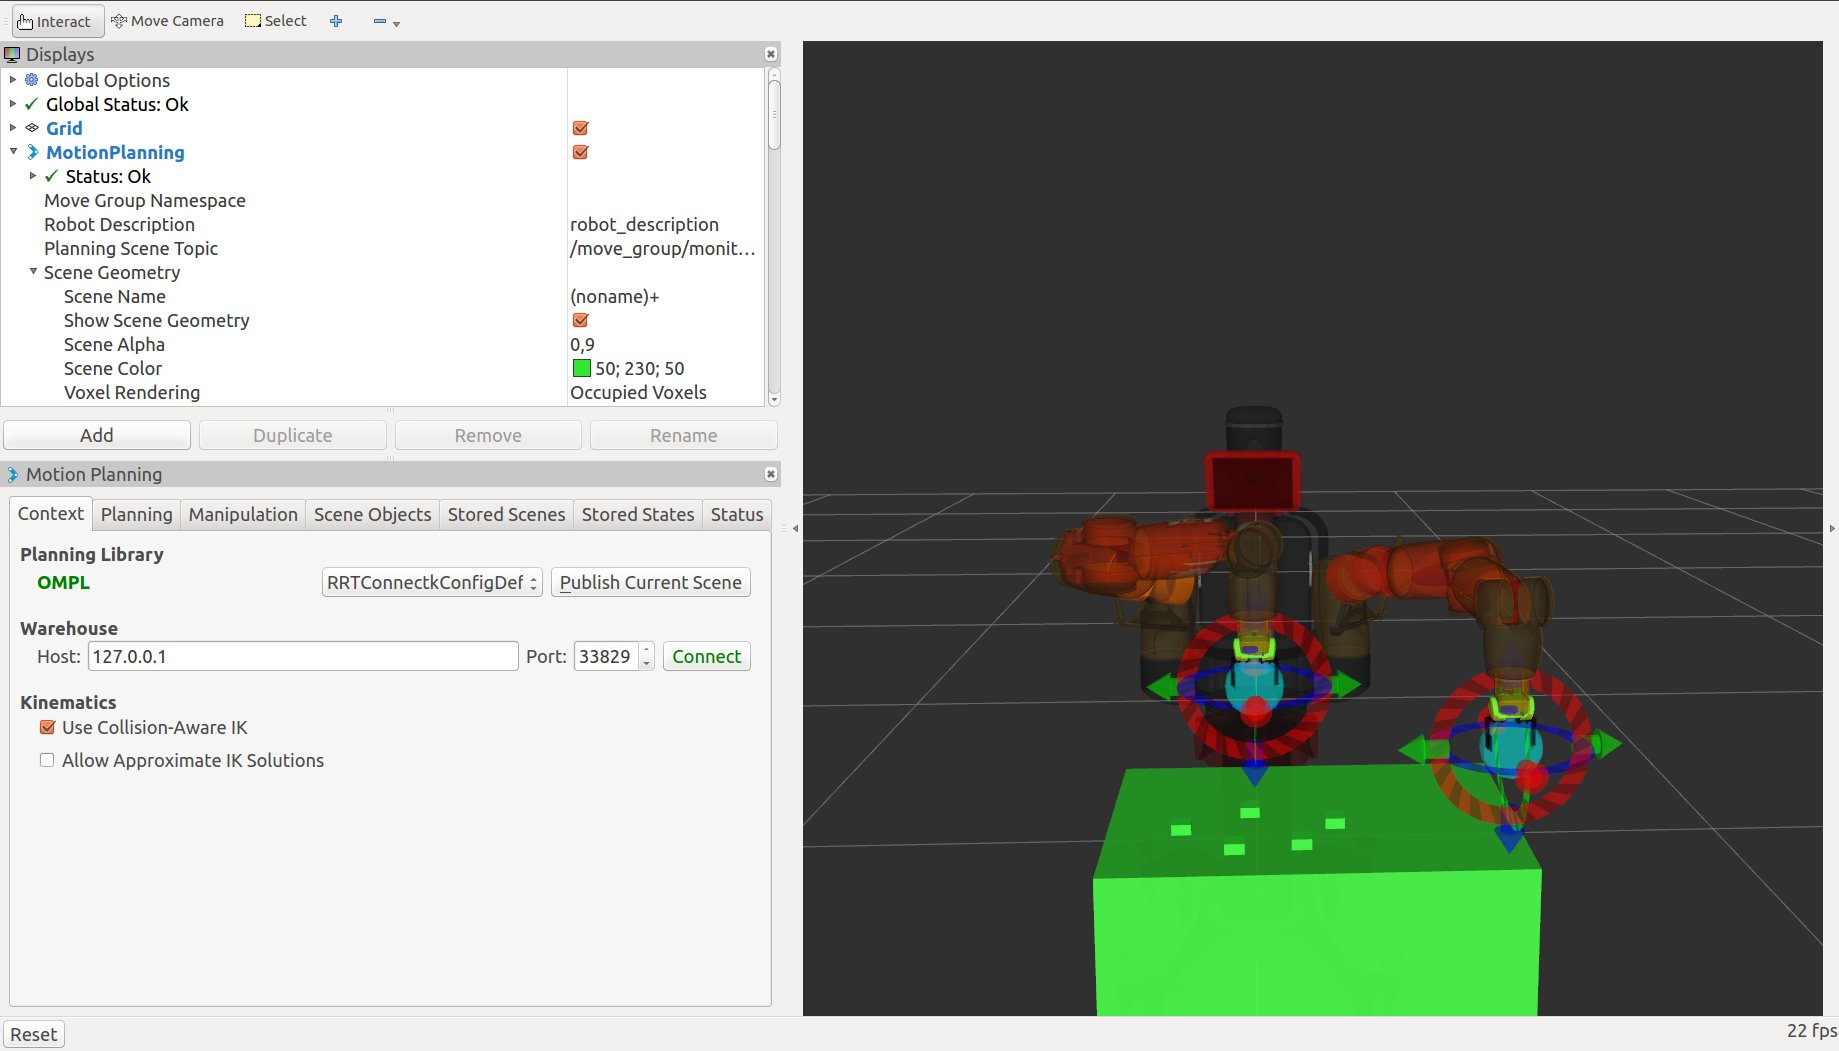
\includegraphics[scale=0.22]{imagenes/initialpos.jpg}
		\caption{Posición inicial de Baxter.}
	\end{figure}
	\item Visión por computador para obtener la imagen de los objetos sobre la mesa o cinta transportadora.
	\item Reconocimiento de objetos.
	\item Si no se reconoce ningún objeto, Baxter no hará nada hasta que sean identificados.
	\item Obtención de información acerca de la posición de los objetos a través de los tópicos de ROS.
	\item Si se trata de clasificación en entorno estático, se procederá a situar el brazo de Baxter entre los objetos con la orientación adecuada para separarlos.
	\item Si, por contrario, se trata de clasificación en entorno dinámico, Baxter llevará la cuña a un punto cercano al punto medio, y conforme los objetos vayan llegando al punto medio obtenido, moverá la cuña con la orientación necesaria para separarlos.
\end{itemize}

\subsection{Restricciones del sistema}

\subsubsection{Restricciones hardware}

\begin{itemize}
	\item El rango de movimiento del brazo derecho (el brazo utilizado) de Baxter es limitado. A la hora de calcular la posición en la que pueden estar los objetos tras un determinado tiempo es posible obtener una posición a la que Baxter no pueda llegar.
	\item No se puede controlar la planificación OMPL realizada por MoveIt!, por lo que no se puede conocer a ciencia cierta cómo va a realizar el movimiento o cuánto va a tardar en realizarlo, siendo la velocidad máxima 1m/s.
	\item Baxter tiene que estar conectado a la corriente.
	\item La cinta transportadora utilizada es estrecha, por lo que no caben muchos objetos.
	\item La cinta transportadora consta de 10 velocidades que se controlan mediante una rueda. 
	\item Es importante disponer de una iluminación suficiente como para que el sistema de reconocimiento identifique los objetos, evitando la aparición de reflejos y artefactos. \\
\end{itemize}

\subsubsection{Restricciones software}
\begin{itemize}
	\item Es necesario realizar este proyecto sobre un directorio RSDK (conexión entre el PC y el robot mediante ROS) de ROS.
	\item En este caso se ha utilizado ROS Kinetic, por lo que sólo se ha podido montar sobre Ubuntu 16.04 LTS, Xenial.
	\item El lenguaje de programación utilizado para la parte de visión por computador será C++, y para el control, Python. \\
\end{itemize}

\subsection{Especificación de casos de uso}
\noindent Los casos de uso describen cómo interactúa un actor con el entorno.\cite{cu} \\
\noindent Las tareas de este proyecto son realizadas por Baxter y el programa de visión por computador.
\begin{itemize}
	\item \textbf{Software de reconocimiento.} Este programa se encarga de procesar la información que llega de las cámaras de Baxter y enviarla ya procesada de nuevo al robot.
	\item \textbf{Baxter.} Se encarga de realizar los movimientos correspondientes utilizando la información que le llega del software de visión. \\
\end{itemize}

\noindent A continuación se muestra el diagrama de casos de uso a seguir para describir cada uno de ellos. \\

\begin{figure}[!h]
	\label{cd:cud}
	 % si queremos la imagen centrada
	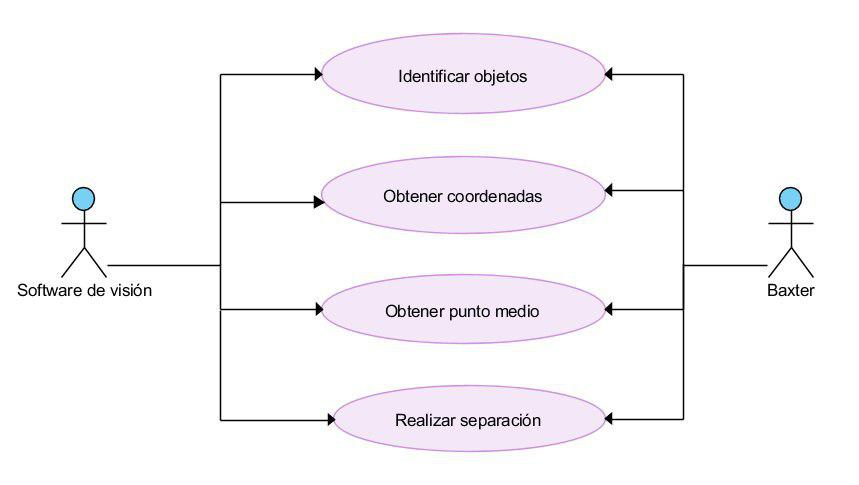
\includegraphics[scale=0.6]{imagenes/cud.jpg}
	\caption{Diagrama de casos de uso.}
\end{figure}

\begin{table}[H]
	\centering
	\begin{tabular}{|p{2.5cm} | p{6cm} | p{5cm} |}
		\hline
		\textbf{Caso de Uso} & Reconocimiento de objetos & \textbf{CU-001} \\
		\hline 
		Actor & \multicolumn{2}{|l|}{Baxter y software de visión} \\
		\hline
		Tipo & \multicolumn{2}{|l|}{Principal | Real} \\
		\hline
		Referencias & RF-001 \ref{cuad:RF-001}, RF-002 \ref{cuad:RF-002}, RF-003 \ref{cuad:RF-003}, RF-004 \ref{cuad:RF-004}, RF-007 \ref{cuad:RF-007}, RNF-001 \ref{cuad:RNF-001}, RNF-002 \ref{cuad:RNF-002} & CU-004 \ref{cuad:CU-002}, CU-003 \ref{cuad:CU-003}, CU-004 \ref{cuad:CU-004}, CU-005 \ref{cuad:CU-005}, CU-006 \ref{cuad:CU-006}, CU-007 \ref{cuad:CU-007}, CU-008 \ref{cuad:CU-007}, CU-008 \ref{cuad:CU-008}, CU-009 \ref{cuad:CU-009} \\
		\hline
		Precondiciones & \multicolumn{2}{|l|}{\parbox{30em}{Los objetos deben estar en el rango de visión de la cámara de Baxter y la iluminación debe permitir reconocerlos.}} \\
		\hline
		Poscondiciones & \multicolumn{2}{|l|}{Se conocerá el centro de los objetos reconocidos en la imagen.}\\
		\hline
		Propósito & \multicolumn{2}{|l|}{\parbox{30em}{Conocer los objetos que hay sobre la mesa o cinta transportadora para clasificarlos.}} \\
		\hline
		Resumen & \multicolumn{2}{|l|}{\parbox{30em}{El software de visión se encarga de reconocer y obtener el punto medio de los objetos que le llegan de la cámara de Baxter.}} \\
		\hline
		
	\end{tabular}
	\caption{Caso de uso CU-001.}
	\label{cuad:CU-001}
\end{table}

\begin{table}[H]
	\centering
	\begin{tabular}{|p{2.5cm} | p{6cm} | p{5cm} |}
		\hline
		\textbf{Caso de Uso} & Obtención del punto medio & \textbf{CU-002} \\
		\hline 
		Actor & \multicolumn{2}{|l|}{Software de visión} \\
		\hline
		Tipo & \multicolumn{2}{|l|}{Secundario | Real} \\
		\hline
		Referencias & RF-003 \ref{cuad:RF-003}, RF-004 \ref{cuad:RF-004}, RF-005 \ref{cuad:RF-005}, RF-007 \ref{cuad:RF-007}, RNF-001 \ref{cuad:RNF-001}, RNF-002 \ref{cuad:RNF-002} & CU-001 \ref{cuad:CU-001}, CU-003 \ref{cuad:CU-003}, CU-004 \ref{cuad:CU-004}, CU-005 \ref{cuad:CU-005}, CU-006 \ref{cuad:CU-006}, CU-007 \ref{cuad:CU-007}, CU-008 \ref{cuad:CU-007}, CU-008 \ref{cuad:CU-008}, CU-009 \ref{cuad:CU-009} \\
		\hline
		Precondiciones & \multicolumn{2}{|l|}{\parbox{30em}{Se deben haber reconocido objetos en la mesa. El algoritmo k-medias debe haberse ejecutado correctamente.}} \\
		\hline
		Poscondiciones & \multicolumn{2}{|l|}{Se conocerá el punto medio de los dos clústers.}\\
		\hline
		Propósito & \multicolumn{2}{|l|}{Conocer el punto medio para situar en él el brazo robótico.} \\
		\hline
		Resumen & \multicolumn{2}{|l|}{\parbox{30em}{El software de visión obtiene a partir del algoritmo k-medias la posición de dos clústers de los que calcula el punto medio.}} \\
		\hline
		
	\end{tabular}
	\caption{Caso de uso CU-002.}
	\label{cuad:CU-002}
\end{table}

\subsubsection{Entorno estático}

\noindent Además de los casos de uso \ref{cuad:CU-001} y \ref{cuad:CU-002}, para realizar la clasificación en entorno estático es necesario el siguiente paso. \\

\begin{table}[H]
	\centering
	\begin{tabular}{|p{2.5cm} | p{6cm} | p{5cm} |}
		\hline
		\textbf{Caso de Uso} & Situar brazo en punto medio en entorno estático & \textbf{CU-003} \\
		\hline 
		Actor & \multicolumn{2}{|l|}{Baxter} \\
		\hline
		Tipo & \multicolumn{2}{|l|}{Primario | Esencial} \\
		\hline
		Referencias & RF-005 \ref{cuad:RF-005}, RF-006 \ref{cuad:RF-006}, RF-007 \ref{cuad:RF-007}, RNF-001 \ref{cuad:RNF-001}, RNF-002 \ref{cuad:RNF-002} & CU-001 \ref{cuad:CU-001}, CU-002 \ref{cuad:CU-002}, CU-004 \ref{cuad:CU-004}, CU-005 \ref{cuad:CU-005} \\
		\hline
		Precondiciones & \multicolumn{2}{|l|}{\parbox{30em}{Haber obtenido el punto medio entre los dos clústers con el algoritmo k-medias.}} \\
		\hline
		Poscondiciones & \multicolumn{2}{|l|}{\parbox{30em}{El brazo robótico se situará en el punto medio entre los clústers con una orientación perpendicular a la que forma la recta que une los dos clústers.}}\\
		\hline
		Propósito & \multicolumn{2}{|l|}{\parbox{30em}{Situar el brazo de Baxter en el punto medio con la orientación necesaria para realizar la clasificación.}} \\
		\hline
		Resumen & \multicolumn{2}{|l|}{\parbox{30em}{Baxter mueve su brazo derecho al punto medio a partir de los datos obtenidos mediante tópicos de ROS.}} \\
		\hline
		
	\end{tabular}
	\caption{Caso de uso CU-003.}
	\label{cuad:CU-003}
\end{table}

\begin{table}[H]
	\centering
	\begin{tabular}{|p{2.5cm} | p{6cm} | p{5cm} |}
		\hline
		\textbf{Caso de Uso} & Rotar paleta en entorno estático & \textbf{CU-004} \\
		\hline 
		Actor & \multicolumn{2}{|l|}{Baxter} \\
		\hline
		Tipo & \multicolumn{2}{|l|}{Primario | Esencial} \\
		\hline
		Referencias & RF-005 \ref{cuad:RF-005}, RF-006 \ref{cuad:RF-006}, RF-007 \ref{cuad:RF-007}, RNF-001 \ref{cuad:RNF-001}, RNF-002 \ref{cuad:RNF-002} & CU-001 \ref{cuad:CU-001}, CU-002 \ref{cuad:CU-002}, CU-003 \ref{cuad:CU-003}, CU-005 \ref{cuad:CU-005} \\
		\hline
		Precondiciones & \multicolumn{2}{|l|}{\parbox{30em}{Haber obtenido el punto medio entre los dos clústers y haber situado en él el gripper con la orientación calculada.}} \\
		\hline
		Poscondiciones & \multicolumn{2}{|l|}{\parbox{30em}{El gripper girará hasta que se encuentre paralelo al eje horizontal.}}\\
		\hline
		Propósito & \multicolumn{2}{|l|}{\parbox{30em}{Rotar el gripper de forma que se pueda realizar más fácilmente la separación.}} \\
		\hline
		Resumen & \multicolumn{2}{|l|}{\parbox{30em}{Se rota el gripper de Baxter de forma que los objetos quedan separados por una recta horizontal.}} \\
		\hline
		
	\end{tabular}
	\caption{Caso de uso CU-004.}
	\label{cuad:CU-004}
\end{table}

\begin{table}[H]
	\centering
	\begin{tabular}{|p{2.5cm} | p{6cm} | p{5cm} |}
		\hline
		\textbf{Caso de Uso} & Separar objetos en entorno estático & \textbf{CU-005} \\
		\hline 
		Actor & \multicolumn{2}{|l|}{Baxter} \\
		\hline
		Tipo & \multicolumn{2}{|l|}{Primario | Esencial} \\
		\hline
		Referencias & RF-005 \ref{cuad:RF-005}, RF-006 \ref{cuad:RF-006}, RF-007 \ref{cuad:RF-007}, RNF-001 \ref{cuad:RNF-001}, RNF-002 \ref{cuad:RNF-002} & CU-001 \ref{cuad:CU-001}, CU-002 \ref{cuad:CU-002}, CU-003 \ref{cuad:CU-003}, CU-004 \ref{cuad:CU-004} \\
		\hline
		Precondiciones & \multicolumn{2}{|l|}{\parbox{30em}{Tener situado el gripper en el punto medio con una orientación paralela al eje horizontal.}} \\
		\hline
		Poscondiciones & \multicolumn{2}{|l|}{\parbox{30em}{El brazo se desplazará en el eje vertical para separar los objetos.}}\\
		\hline
		Propósito & \multicolumn{2}{|l|}{\parbox{30em}{Separar los objetos mediante movimientos en el eje vertical de Baxter.}} \\
		\hline
		Resumen & \multicolumn{2}{|l|}{\parbox{30em}{Desplazar el brazo arriba y abajo en el eje vertical separando los objetos conforme a color y posición.}} \\
		\hline
		
	\end{tabular}
	\caption{Caso de uso CU-005.}
	\label{cuad:CU-005}
\end{table}

\subsubsection{Entorno dinámico}
\noindent Para realizar la clasificación con una cuña como herramienta y una cinta transportadora sobre la que se sitúan los objetos, además del caso de uso \ref{cuad:CU-001}, es necesario lo siguiente. \\

\begin{table}[H]
	\centering
	\begin{tabular}{|p{2.5cm} | p{6cm} | p{5cm} |}
		\hline
		\textbf{Caso de Uso} & Cálculo de la velocidad en entorno dinámico & \textbf{CU-006} \\
		\hline 
		Actor & \multicolumn{2}{|l|}{Software} \\
		\hline
		Tipo & \multicolumn{2}{|l|}{Secundario | Real} \\
		\hline
		Referencias & RF-004 \ref{cuad:RF-004}, RF-005 \ref{cuad:RF-005}, RF-006 \ref{cuad:RF-006}, RF-007 \ref{cuad:RF-007}, RNF-001 \ref{cuad:RNF-001}, RNF-002 \ref{cuad:RNF-002} & CU-001 \ref{cuad:CU-001}, CU-002 \ref{cuad:CU-002}, CU-007 \ref{cuad:CU-007}, CU-008 \ref{cuad:CU-008}, CU-009 \ref{cuad:CU-009} \\
		\hline
		Precondiciones & \multicolumn{2}{|l|}{\parbox{30em}{Haber obtenido el punto medio entre los dos clústers en dos ocasiones.}} \\
		\hline
		Poscondiciones & \multicolumn{2}{|l|}{\parbox{30em}{Se conocerá la velocidad media a la que van los objetos sobre la cinta transportadora.}}\\
		\hline
		Propósito & \multicolumn{2}{|l|}{\parbox{30em}{Obtener la velocidad a la que van los objetos para realizar la separación.}} \\
		\hline
		Resumen & \multicolumn{2}{|l|}{\parbox{30em}{Se obtiene la posición del punto medio entre los dos clústers en dos ocasiones, una al principio y otra un tiempo después y se calcula la velocidad que llevan los objetos.}} \\
		\hline
		
	\end{tabular}
	\caption{Caso de uso CU-006.}
	\label{cuad:CU-006}
\end{table}

\begin{table}[H]
	\centering
	\begin{tabular}{|p{2.5cm} | p{6cm} | p{5cm} |}
		\hline
		\textbf{Caso de Uso} & Situar brazo en posición cercana al punto medio en entorno dinámico & \textbf{CU-007} \\
		\hline 
		Actor & \multicolumn{2}{|l|}{Baxter} \\
		\hline
		Tipo & \multicolumn{2}{|l|}{Primario | Esencial} \\
		\hline
		Referencias & RF-005 \ref{cuad:RF-005}, RF-006 \ref{cuad:RF-006}, RF-007 \ref{cuad:RF-007}, RNF-001 \ref{cuad:RNF-001}, RNF-002 \ref{cuad:RNF-002} & CU-001 \ref{cuad:CU-001}, CU-002 \ref{cuad:CU-002}, CU-006 \ref{cuad:CU-006}, CU-008 \ref{cuad:CU-008}, CU-009 \ref{cuad:CU-009} \\
		\hline
		Precondiciones & \multicolumn{2}{|l|}{\parbox{30em}{Haber obtenido el último valor de punto medio entre los dos clústers y la velocidad a la que van los objetos.}} \\
		\hline
		Poscondiciones & \multicolumn{2}{|l|}{\parbox{30em}{El brazo robótico se situará en un punto cercano al punto medio aumentando la rotación del gripper.}} \\
		\hline
		Propósito & \multicolumn{2}{|l|}{\parbox{30em}{Mover el brazo a un punto cercano al punto medio para realizar el barrido necesario para clasificar los objetos.}} \\
		\hline
		Resumen & \multicolumn{2}{|l|}{\parbox{30em}{Baxter mueve su brazo derecho al punto calculado con un valor de orientación más alto que el calculado para el punto medio.}} \\
		\hline
		
	\end{tabular}
	\caption{Caso de uso CU-007.}
	\label{cuad:CU-007}
\end{table}

\begin{table}[H]
	\centering
	\begin{tabular}{|p{2.5cm} | p{6cm} | p{5cm} |}
		\hline
		\textbf{Caso de Uso} & Situar brazo en punto medio en entorno dinámico & \textbf{CU-008} \\
		\hline 
		Actor & \multicolumn{2}{|l|}{Baxter} \\
		\hline
		Tipo & \multicolumn{2}{|l|}{Primario | Esencial} \\
		\hline
		Referencias & RF-005 \ref{cuad:RF-005}, RF-006 \ref{cuad:RF-006}, RF-007 \ref{cuad:RF-007}, RNF-001 \ref{cuad:RNF-001}, RNF-002 \ref{cuad:RNF-002} & CU-001 \ref{cuad:CU-001}, CU-002 \ref{cuad:CU-002}, CU-006 \ref{cuad:CU-006}, CU-007 \ref{cuad:CU-007}, CU-009 \ref{cuad:CU-009} \\
		\hline
		Precondiciones & \multicolumn{2}{|l|}{\parbox{30em}{El gripper debe estar situado en un punto cercano al punto medio.}} \\
		\hline
		Poscondiciones & \multicolumn{2}{|l|}{\parbox{30em}{Baxter mueve el brazo hacia el último punto medio obtenido con la orientación necesaria para realizar la separación.}} \\
		\hline
		Propósito & \multicolumn{2}{|l|}{\parbox{30em}{Mover el brazo al punto medio para realizar la separación.}} \\
		\hline
		Resumen & \multicolumn{2}{|l|}{\parbox{30em}{Baxter mueve su brazo derecho al punto medio con la orientación adecuada para que los objetos queden separados.}} \\
		\hline
		
	\end{tabular}
\caption{Caso de uso CU-008}
\label{cuad:CU-008}
\end{table}

\begin{table}[H]
	\centering
	\begin{tabular}{|p{2.5cm} | p{6cm} | p{5cm} |}
		\hline
		\textbf{Caso de Uso} & Sacudida de objetos en entorno dinámico & \textbf{CU-009} \\
		\hline 
		Actor & \multicolumn{2}{|l|}{Baxter} \\
		\hline
		Tipo & \multicolumn{2}{|l|}{Primario | Esencial} \\
		\hline
		Referencias & RF-005 \ref{cuad:RF-005}, RF-006 \ref{cuad:RF-006}, RF-007 \ref{cuad:RF-007}, RNF-001 \ref{cuad:RNF-001}, RNF-002 \ref{cuad:RNF-002} & CU-001 \ref{cuad:CU-001}, CU-002 \ref{cuad:CU-002}, CU-006 \ref{cuad:CU-006}, CU-007 \ref{cuad:CU-007}, CU-008 \ref{cuad:CU-008} \\
		\hline
		Precondiciones & \multicolumn{2}{|l|}{\parbox{30em}{El brazo se encuentra en el punto medio en el que separa los objetos.}} \\
		\hline
		Poscondiciones & \multicolumn{2}{|l|}{\parbox{30em}{Baxter moverá el brazo con la misma orientación que tenía en el eje vertical para separar los objetos más satisfactoriamente.}} \\
		\hline
		Propósito & \multicolumn{2}{|l|}{\parbox{30em}{Realizar movimientos verticales con la posición actual del gripper para separar más rápido los objetos.}} \\
		\hline
		Resumen & \multicolumn{2}{|l|}{\parbox{30em}{Se mueve el brazo derecho en su posición actual en el eje vertical separando más rápidamente los objetos.}} \\
		\hline
		
	\end{tabular}
	\caption{Caso de uso CU-009.}
	\label{cuad:CU-009}
\end{table}

\subsection{Especificación de requisitos}
\noindent Los requisitos pueden ser clasificados en funcionales o no funcionales. Los funcionales se refieren a cualquier comportamiento que esté directamente relacionado con el funcionamiento del sistema, mientras que los requisitos no funcionales especifican cómo debe comportarse el sistema. \\

\subsubsection{Requisitos funcionales}
\begin{table}[H]
	\centering
	\begin{tabular}{|p{2cm} | p{1.5cm} | p{2cm} | p{1.7cm} | p{2cm} | p{2cm} |}
		\hline
		\multicolumn{6}{|c|}{\textbf{REQUISITO DEL SISTEMA}} \\ 
		\hline
		\textbf{ID} & RF-001 & & \textbf{Fuente} & \multicolumn{2}{c|}{CU-001} \\
		\hline
		\textbf{Nombre} & \multicolumn{5}{l|}{Reconocimiento de objetos} \\
		\hline
		\textbf{Descripción} & \multicolumn{5}{l|}{\parbox{30em}{Se obtienen imágenes de los objetos situados en la mesa, visibles a la cámara del brazo derecho de Baxter.}} \\
		\hline
		\textbf{Prioridad} & Alta & \textbf{Necesidad} & Esencial & \textbf{Estabilidad} & Estable \\
		\hline		
	\end{tabular}
	\caption{Requisito funcional RF-001.}
	\label{cuad:RF-001}
\end{table}

\begin{table}[H]
	\centering
	\begin{tabular}{|p{2cm} | p{1.5cm} | p{2cm} | p{1.7cm} | p{2cm} | p{2cm} |}
		\hline
		\multicolumn{6}{|c|}{\textbf{REQUISITO DEL SISTEMA}} \\ 
		\hline
		\textbf{ID} & RF-002 & & \textbf{Fuente} & \multicolumn{2}{c|}{CU-001} \\
		\hline
		\textbf{Nombre} & \multicolumn{5}{l|}{Recortar la imagen} \\
		\hline
		\textbf{Descripción} & \multicolumn{5}{l|}{\parbox{30em}{Recortar la imagen para asegurar que la visión no reconoce otros objetos distintos a los que hay en la cinta.}} \\
		\hline
		\textbf{Prioridad} & Alta & \textbf{Necesidad} & Deseable & \textbf{Estabilidad} & Estable \\
		\hline		
	\end{tabular}
	\caption{Requisito funcional RF-002.}
	\label{cuad:RF-002}
\end{table}

\begin{table}[H]
	\centering
	\begin{tabular}{|p{2cm} | p{1.5cm} | p{2cm} | p{1.7cm} | p{2cm} | p{2cm} |}
		\hline
		\multicolumn{6}{|c|}{\textbf{REQUISITO DEL SISTEMA}} \\ 
		\hline
		\textbf{ID} & RF-003 & & \textbf{Fuente} & \multicolumn{2}{c|}{CU-001} \\
		\hline
		\textbf{Nombre} & \multicolumn{5}{l|}{Identificar objetos} \\
		\hline
		\textbf{Descripción} & \multicolumn{5}{l|}{El sistema identifica los objetos de colores situados en la escena.} \\
		\hline
		\textbf{Prioridad} & Alta & \textbf{Necesidad} & Esencial & \textbf{Estabilidad} & Estable \\
		\hline		
	\end{tabular}
	\caption{Requisito funcional RF-003.}
	\label{cuad:RF-003}
\end{table}

\begin{table}[H]
	\centering
	\begin{tabular}{|p{2cm} | p{1.5cm} | p{2cm} | p{1.7cm} | p{2cm} | p{2cm} |}
		\hline
		\multicolumn{6}{|c|}{\textbf{REQUISITO DEL SISTEMA}} \\ 
		\hline
		\textbf{ID} & RF-004 & & \textbf{Fuente} & \multicolumn{2}{c|}{CU-001} \\
		\hline
		\textbf{Nombre} & \multicolumn{5}{l|}{Obtener coordenadas} \\
		\hline
		\textbf{Descripción} & \multicolumn{5}{l|}{\parbox{30em}{El sistema obtiene el centro de los objetos situados en la escena.}} \\
		\hline
		\textbf{Prioridad} & Alta & \textbf{Necesidad} & Esencial & \textbf{Estabilidad} & Inestable \\
		\hline		
	\end{tabular}
	\caption{Requisito funcional RF-004.}
	\label{cuad:RF-004}
\end{table}

\begin{table}[H]
	\centering
	\begin{tabular}{|p{2cm} | p{1.5cm} | p{2cm} | p{1.7cm} | p{2cm} | p{2cm} |}
		\hline
		\multicolumn{6}{|c|}{\textbf{REQUISITO DEL SISTEMA}} \\ 
		\hline
		\textbf{ID} & RF-005 & & \textbf{Fuente} & \multicolumn{2}{c|}{CU-001} \\
		\hline
		\textbf{Nombre} & \multicolumn{5}{l|}{Obtener punto medio y orientación} \\
		\hline
		\textbf{Descripción} & \multicolumn{5}{l|}{\parbox{30em}{El sistema obtiene, a partir del algoritmo k-medias, el centro entre los dos clústers. A partir de los dos puntos de los clústers calcula la recta que forman y la pendiente perpendicular a esta, que será la orientación asociada a la separación.}} \\
		\hline
		\textbf{Prioridad} & Alta & \textbf{Necesidad} & Esencial & \textbf{Estabilidad} & Inestable \\
		\hline		
	\end{tabular}
	\caption{Requisito funcional RF-005.}
	\label{cuad:RF-005}
\end{table}

\begin{table}[H]
	\centering
	\begin{tabular}{|p{2cm} | p{1.5cm} | p{2cm} | p{1.7cm} | p{2cm} | p{2cm} |}
		\hline
		\multicolumn{6}{|c|}{\textbf{REQUISITO DEL SISTEMA}} \\ 
		\hline
		\textbf{ID} & RF-006 & & \textbf{Fuente} & \multicolumn{2}{c|}{CU-001} \\
		\hline
		\textbf{Nombre} & \multicolumn{5}{l|}{Cargar posición inicial} \\
		\hline
		\textbf{Descripción} & \multicolumn{5}{l|}{\parbox{30em}{Baxter pone sus extremidades en la posición inicial (figura \ref*{cd:ip}).}} \\
		\hline
		\textbf{Prioridad} & Alta & \textbf{Necesidad} & Esencial & \textbf{Estabilidad} & Estable \\
		\hline		
	\end{tabular}
	\caption{Requisito funcional RF-006.}
	\label{cuad:RF-006}
\end{table}

\begin{table}[H]
	\centering
	\begin{tabular}{|p{2cm} | p{1.5cm} | p{2cm} | p{1.7cm} | p{2cm} | p{2cm} |}
		\hline
		\multicolumn{6}{|c|}{\textbf{REQUISITO DEL SISTEMA}} \\ 
		\hline
		\textbf{ID} & RF-007 & & \textbf{Fuente} & \multicolumn{2}{c|}{CU-001} \\
		\hline
		\textbf{Nombre} & \multicolumn{5}{l|}{Mostrar escena} \\
		\hline
		\textbf{Descripción} & \multicolumn{5}{l|}{\parbox{30em}{Mediante tópicos de ROS se obtiene la escena que Baxter ve en cada momento, delineando los objetos reconocidos.}} \\
		\hline
		\textbf{Prioridad} & Media & \textbf{Necesidad} & Deseable & \textbf{Estabilidad} & Inestable \\
		\hline		
	\end{tabular}
	\caption{Requisito funcional RF-007.}
	\label{cuad:RF-007}
\end{table}

\subsubsection{Requisitos no funcionales}

\begin{table}[H]
	\centering
	\begin{tabular}{|p{2cm} | p{1.5cm} | p{2cm} | p{1.7cm} | p{2cm} | p{2cm} |}
		\hline
		\multicolumn{6}{|c|}{\textbf{REQUISITO DEL SISTEMA}} \\ 
		\hline
		\textbf{ID} & RNF-001 & & \textbf{Fuente} & \multicolumn{2}{c|}{CU-001} \\
		\hline
		\textbf{Nombre} & \multicolumn{5}{l|}{Iluminación adecuada} \\
		\hline
		\textbf{Descripción} & \multicolumn{5}{l|}{\parbox{30em}{La luz debe ser lo bastante intensa como para ver los objetos pero para que estos no la reflejen.}} \\ 
		\hline
		\textbf{Prioridad} & Media & \textbf{Necesidad} & Deseable & \textbf{Estabilidad} & Inestable \\
		\hline		
	\end{tabular}
	\caption{Requisito no funcional RNF-001.}
	\label{cuad:RNF-001}
\end{table}

\begin{table}[H]
	\centering
	\begin{tabular}{|p{2cm} | p{1.5cm} | p{2cm} | p{1.7cm} | p{2cm} | p{2cm} |}
		\hline
		\multicolumn{6}{|c|}{\textbf{REQUISITO DEL SISTEMA}} \\ 
		\hline
		\textbf{ID} & RNF-002 & & \textbf{Fuente} & \multicolumn{2}{c|}{CU-001} \\
		\hline
		\textbf{Nombre} & \multicolumn{5}{l|}{Utilizar a Baxter} \\
		\hline
		\textbf{Descripción} & \multicolumn{5}{l|}{\parbox{30em}{En este proyecto el robot utilizado es Baxter.}} \\
		\hline
		\textbf{Prioridad} & Alta & \textbf{Necesidad} & Esencial & \textbf{Estabilidad} & Estable \\
		\hline		
	\end{tabular}
	\caption{Requisito no funcional RNF-002.}
	\label{cuad:RNF-002}
\end{table}

\newpage
\section{Diseño}

\noindent Para especificar la estructura que se ha seguido en el diseño del proyecto, se muestra un diagrama de flujo vertical en el que se incluye tanto el programa encargado de la clasificación en entorno estático como el encargado de la clasificación en entorno dinámico.\\
\noindent Seguidamente, se expondrán los principales módulos responsables de realizar las tareas especificadas. \\

\begin{figure}[H]
	\label{cd:flowd}
	\centering % si queremos la imagen centrada
	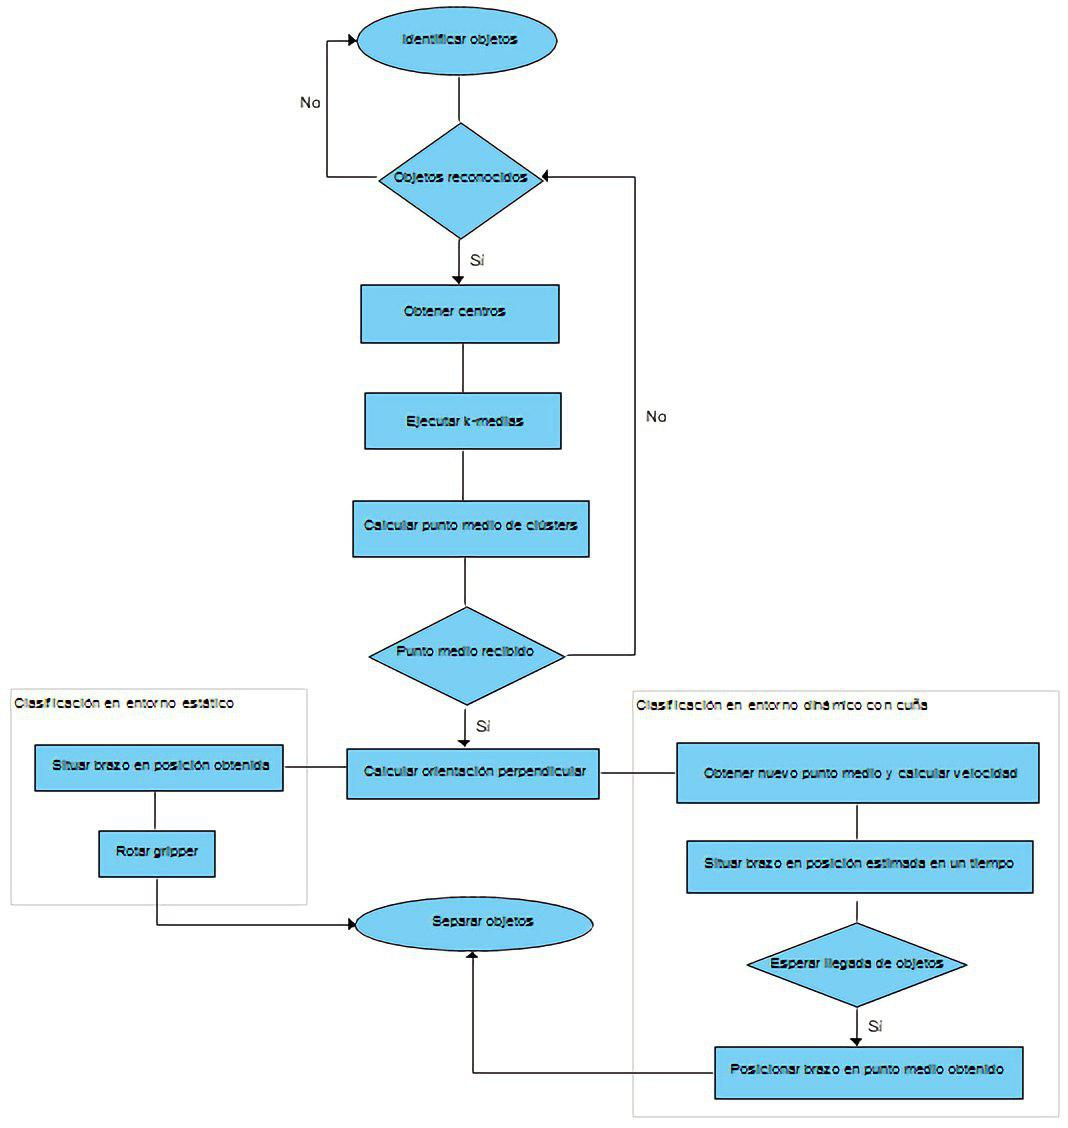
\includegraphics[scale=0.5]{imagenes/flowd.jpg}
	\caption{Diagrama de flujo.}
\end{figure}

\begin{itemize}
	\item \textbf{Módulo de reconocimiento.} Este es el que se encargará de identificar los objetos, procesar los datos y enviarlos al módulo de control de Baxter.\\
	\item \textbf{Módulo de control de Baxter.} La función de este módulo será realizar los movimientos y cálculos necesarios para separar los objetos. Además se incluye la planificación y ejecución de trayectorias. \\
\end{itemize}

\subsection{Módulo de reconocimiento}
\noindent Este módulo incorpora la visión por computador. Lo componen: \\

\begin{itemize}
	\item \textit{GetPosition}. Es la función encargada de obtener las coordenadas del centro de los objetos en la imagen.
	\item \textit{Get3DPos}. Se encarga de obtener las coordenadas en el mundo real a partir de las coordenadas de la imagen.
	\item \textit{GetRealPos}. A partir de las coordenadas dadas por \textit{Get3DPos}, obtiene el centro de los objetos en el mundo real.
	\item \textit{ImageCallBack}. Cada vez que se recibe una imagen, esta función se encarga de procesarla y enviar los datos a través de ROS al módulo de control de Baxter.
\end{itemize}

\subsection{Módulo de control de Baxter}
\noindent Como se dijo anteriormente, este es el módulo que se encargará del control sobre el robot, además de realizar algunos cálculos necesarios para poder clasificar los objetos. \\

\begin{itemize}
	\item \textit{baxter\_interface}: este nodo es el encargado de definir los brazos y \textit{grippers} de Baxter en Python. Para ello, se utilizan las siguientes órdenes: \\
	
	- \textit{right\_arm = baxter\_interface.limb.Limb('right')}
	
	- \textit{right\_gripper = baxter\_interface.Gripper('right')}\\
	
	Además, una vez se han definido los \textit{grippers}, estos se pueden calibrar y abrir o cerrar. \\
	
	
	\item \textit{moveit\_commander}: este es el nodo de MoveIt! para Python que se encargará de realizar los movimientos en Baxter y planificar la escena para detectar colisiones o utilizar RViz para moverlo. \\
	
	- \textit{p = PlanningSceneInterface(``base")}. Esta orden inicializa la escena en MoveIt!.\\
	- \textit{arms\_group = MoveGroupInterface(``both\_arms", "base")}. Se encarga de inicializar ambos brazos en la escena. \\
	- \textit{rightarm\_group = MoveGroupInterface(``right\_arm'', ``base")}. Inicializa el brazo derecho en la escena. Se realiza análogamente para el izquierdo.\\
	- \textit{rightarm\_group.moveToPose \\(position, ``right\_gripper'', max\_velocity\_scaling\_factor=1, plan\_only=False)}. Esta orden es la encargada de realizar los movimientos, en este caso, el brazo derecho se moverá hasta la posición ``\textit{position}'' con una velocidad máxima de 1 m/s. \\
	
	\item \textit{rotate\_pose\_by\_euler\_angles}: es la función encargada de rotar los \textit{grippers} a la orientación establecida.\\
\end{itemize}